\secnumbersection{PROPUESTA DE SOLUCIÓN}
\setcounter{secnumdepth}{4}
\setcounter{tocdepth}{4}
\makeatletter
\renewcommand\paragraph{\@startsection{paragraph}{4}{\z@}%
  {1.5ex \@plus .5ex \@minus .2ex}%   % espacio antes
  {0.8ex \@plus .2ex}%                 % espacio después
  {\normalfont\normalsize\bfseries}}  % estilo
\makeatother



Esta propuesta abarca la evolución de \textbf{DRAFTS} \cite{zhang2024drafts} desde un prototipo de investigación para la detección y clasificación de FRBs, hacia un \textit{pipeline} 
\textbf{productivo, robusto y eficiente} diseñado para detectar y clasificar transientes de radio y FRBs de forma sencilla y fácil para el astrónomo. Esta transformación arquitectónica no se limita a 
mejoras incrementales, sino que además establece una \textbf{extensión fundamental para regímenes de alta frecuencia} que expande significativamente las capacidades de 
detección en el espectro milimétrico.

De ahora en adelante, a esta nueva versión de DRAFTS le llamaremos DRAFTS++, que es básicamente toda esta memoria.

\subsection{Vista General: Dos Grandes Bloques de Contribución a los pipelines astronómicos de FRBs}

Esta propuesta se estructura en \textbf{dos grandes bloques} que abordan desafíos complementarios en la detección de FRBs:

\begin{itemize}
    \item \textbf{Bloque 1: DRAFTS++: Pipeline astronómico E2E, Productivo, Robusto y Eficiente}: Este bloque aborda la transformación del prototipo DRAFTS hacia un sistema productivo capaz de operar en entornos observacionales reales. Este bloque incluye la refactorización arquitectónica completa; la implementación de procesamiento eficiente por \emph{chunks}; la gestión eficiente de memoria y recursos; la trazabilidad completa; y artefactos de salida estandarizados.

    \item \textbf{Bloque 2: DRAFTS++: Extensión a Alta Frecuencia - Cuatro Líneas de Investigación:} Este bloque explora estrategias metodológicas para extender las capacidades de detección hacia regímenes de alta frecuencia (30-100 GHz), donde las firmas dispersivas tradicionales se atenúan significativamente. Este bloque presenta cuatro líneas de investigación complementarias que abordan diferentes aspectos del desafío de detección en el espectro milimétrico.
\end{itemize}

\subsection{Bloque 1: DRAFTS++: Pipeline astronómico E2E, Productivo, Robusto y Eficiente}

Como ya se mencionó anteriormente, aquí se contempla la transformación fundamental del prototipo DRAFTS hacia un sistema productivo capaz de operar en entornos observacionales reales. La evolución desde un prototipo de investigación hacia un sistema productivo requiere una transformación arquitectónica fundamental que aborde las limitaciones inherentes del código base original.

\subsubsection{Desafíos y limitaciones de DRAFTS: diagnóstico claro del prototipo original.}

DRAFTS es un "pseudo-pipeline", mas cerca a ser un prototipo que un software astronomico, pero ojo, en cuanto a lo que son los modelos de redes neuronales estos son modelos de deteccion y clasificacion de FRBs robustos y completamente funcionales, el problema surge al rededor de estos modelos, pues DRAFTS presenta una estructura monolítica con scripts independientes optimizados para condiciones de laboratorio controladas pero incapaces de manejar la variabilidad operacional de entornos observacionales reales. Más que limitaciones incrementales, el código original no constituye un \emph{pipeline} operativo: la búsqueda en datos reales se materializa en programas separados que el usuario debe ejecutar y parametrizar manualmente. No existe un punto de entrada unificado, una interfaz de línea de comandos ni un sistema de configuración versionado; el flujo exige editar variables en el código (rutas, umbrales, \textit{checkpoints}, tamaños de bloque, DM, etc.) y correr etapas desconectadas sin orquestación. El propio \texttt{README} instruye a "modificar la ruta de datos y de guardado y ejecutar el archivo", lo que evidencia la ausencia de un flujo automatizado de extremo a extremo que, con un único \emph{input}, entregue resultados reproducibles, directos y simples para el usuario astrónomo.

En la ingesta de datos se observan supuestos instrumentales rígidos. El lector de PSRFITS asume un esquema específico propio de FAST/GBT, y el repositorio indica explícitamente que para otros telescopios se deben "modificar" funciones internas. No hay detección automática de formato ni un análisis robusto de encabezados; los parámetros observacionales se derivan parcialmente con constantes implícitas y números mágicos (p.ej., factores de decimado temporal y espectral), además de correcciones ad hoc como la inversión del eje de frecuencia o normalizaciones mín--máx. Tampoco se calculan marcas temporales precisas a partir de los \emph{headers}, por lo que los tiempos de arribo son relativos y no trazables de manera consistente dentro del archivo ni interoperables con análisis posteriores.

La gestión de datos y memoria es frágil para observaciones prolongadas. El procesamiento es monolítico sobre bloques grandes construidos concatenando archivos contiguos en memoria, y para completar las ventanas de dedispersión en los bordes se recurre a relleno sintético con ruido aleatorio cuando faltan muestras, alterando la estadística de fondo y comprometiendo la validez científica en condiciones reales. La dedispersión GPU (\texttt{numba.cuda}) opera sobre tensores completos de DM--tiempo sin un planificador de \textit{chunking} que respete un presupuesto de memoria; no hay telemetría ni control de uso de VRAM, limpieza sistemática, \textit{fallback} a CPU ante \emph{out-of-memory} o manejo robusto de errores. Esta combinación limita la estabilidad y escalabilidad del sistema cuando la duración, el ancho de banda o la resolución crecen.

La extracción y validación de candidatos carecen de un esqueleto unificado. La detección obtiene cajas en DM--tiempo, pero el filtrado posterior es heurístico (p.ej., exigir \texttt{DM > 20}) y la clasificación está desacoplada en un programa distinto que dedispersa a un DM fijo predefinido, sin realimentación del detector. No existe un validador físico común (coherencia por sub--bandas, verificación de DM positivo con incertidumbre acotada, consistencia temporal entre ventanas) ni mecanismos de desduplicación de eventos entre \emph{slices} y archivos. Las salidas se limitan a imágenes y algunos archivos \texttt{.npy} por bloque; no se generan artefactos estandarizados (CSV/Parquet con metadatos completos), ni resúmenes por ejecución, ni firmas de modelos y datos que habiliten trazabilidad y auditoría. La ausencia de \emph{logging} estructurado y de semillas controladas impide reproducir resultados de manera fiable.

En operación y extensibilidad, los modelos se cargan desde rutas relativas y su presencia es un prerrequisito tácito; si faltan, el programa simplemente falla sin orientación al usuario. No hay empaquetado ni instalación como librería, pruebas automatizadas, ni documentación de un flujo end--to--end; el entrenamiento existe, pero la integración con la búsqueda es manual. La compatibilidad multi--banda y el tratamiento de polarización son limitados (se promedian canales y polarizaciones tempranamente), y no existe un mecanismo para seleccionar estrategias de búsqueda según condiciones físicas (resolución temporal, rango de frecuencias, SNR, disponibilidad de Stokes). 

En suma, a pesar de contar con modelos de detección y clasificación bien entrenados, el prototipo carece del software de \emph{pipeline} que permita, con un único \emph{input}, obtener resultados directos, sencillos y trazables en un entorno observacional real, es de ahi que nace DRAFTS++.

\subsubsection{Construccion de un Pipeline End-to-End Modular y Escalable: DRAFTS++}

% Construcción y Diseño de DRAFTS++

A continuación, se procede a explicar y narrar la transformación arquitectónica fundamental que sufrió DRAFTS para ser DRAFTS++. 

La evolución desde los scripts monolíticos hacia un sistema modular escalable constituye una contribución arquitectónica fundamental que establece las bases para operaciones productivas a gran escala. Esta transformación implementa una arquitectura modular con componentes especializados que establecen separación clara de responsabilidades e interfaces estandarizadas. La reestructuración arquitectónica elimina las limitaciones inherentes del prototipo original, caracterizado por scripts independientes sin integración coherente, y establece un flujo de datos unidireccional que garantiza consistencia operacional y facilita mantenimiento y extensibilidad del sistema.

Para materializar todo esto, DRAFTS++ se gestiona en \textbf{etapas encadenadas} que transforman los datos desde la ingesta hasta los artefactos finales, y en \textbf{servicios transversales} que aseguran orden, reproducibilidad y operación continua. Las etapas (ingesta, preprocesamiento, modelos, detección, análisis y visualización) reciben entradas bien definidas y devuelven salidas contratadas; los transversales (\texttt{core/}, \texttt{config/}, \texttt{logging/}, \texttt{scripts/}) proveen orquestación, configuración validada, trazabilidad y puntos de entrada. Este enfoque divide el problema en unidades comprensibles y sustituibles, habilitando evolución independiente sin comprometer la coherencia global.

La \textbf{visión operativa} se resume en cuatro ejes: (i) un uso \textbf{productivo} del sistema, con punto de entrada único, configuración centralizada y artefactos estandarizados; (ii) \textbf{robustez} frente a formatos y condiciones instrumentales diversas mediante autodetección, validaciones físicas/temporales y recuperación guiada ante fallos; (iii) \textbf{eficiencia} por streaming con presupuestos de memoria explícitos, limpieza determinística y uso controlado de GPU; y (iv) \textbf{replicabilidad/auditoría} garantizada por semillas fijas, versiones y firmas de datos/modelos y \emph{logging} estructurado.

Para sostener estos ejes se adoptan \textbf{principios arquitectónicos} claros: modularidad y separación de responsabilidades; flujo de datos estrictamente unidireccional con \textbf{contratos} entre etapas (geometrías, metadatos, candidatos); configuración validada con valores por defecto seguros; \textbf{streaming y \emph{chunking}} con solapamiento físico y continuidad temporal verificada; \textbf{observabilidad} mediante métricas y estados normalizados; y \textbf{outputs estandarizados} que facilitan consumo externo y auditoría científica.

Para entender mejor esto, podemos ver la Figura \ref{fig:workflow-src}, la cual resume el flujo principal y los soportes transversales del pipeline DRAFTS++, que guían el orden de este Bloque 1.

\begin{figure}[H]
\centering
\begingroup\shorthandoff{<>}% desactivar atajos de babel para < y > dentro de TikZ
\resizebox{\textwidth}{!}{%
\begin{tikzpicture}[
    node distance=1.0cm and 1.6cm,
    stage/.style={rectangle, draw, fill=blue!20, text width=2.7cm, text centered, minimum height=0.7cm, font=\small},
    support/.style={rectangle, draw, fill=gray!20, text width=2.7cm, text centered, minimum height=0.6cm, font=\small, rounded corners},
    arrow/.style={-Stealth, thick, shorten >=2pt}
]

% Flujo principal por etapas (de izquierda a derecha)
\node[stage] (in) {input/\\Ingesta};
\node[stage, right=of in] (pp) {preprocessing/\\Preprocesamiento};
\node[stage, right=of pp] (md) {models/\\Modelos};
\node[stage, right=of md] (dt) {detection/\\Detección};
\node[stage, right=of dt] (an) {analysis/\\Análisis};
\node[stage, right=of an] (vz) {visualization/\\Visualización};
\node[stage, right=of vz] (out) {output/\\Artefactos};

\draw[arrow] (in) -- (pp);
\draw[arrow] (pp) -- (md);
\draw[arrow] (md) -- (dt);
\draw[arrow] (dt) -- (an);
\draw[arrow] (an) -- (vz);
\draw[arrow] (vz) -- (out);

% Módulos transversales de soporte (debajo)
\node[support, below=3.2cm of md] (core) {core/\\Utilidades y Orquestación};
\node[support, left=1.8cm of core] (cfg) {config/\\Configuración};
\node[support, right=1.8cm of core] (log) {logging/\\Registro};
\node[support, below=2.2cm of core] (scr) {scripts/\\CLI y Entradas};

% Conexiones (líneas punteadas) desde soporte a etapas
% Conexiones (desde borde superior de soporte al borde inferior de etapas)
\draw[arrow, dashed] (core.north) -- (in.south);
\draw[arrow, dashed] (core.north) -- (pp.south);
\draw[arrow, dashed] (core.north) -- (md.south);
\draw[arrow, dashed] (core.north) -- (dt.south);
\draw[arrow, dashed] (core.north) -- (an.south);
\draw[arrow, dashed] (core.north) -- (vz.south);

\draw[arrow, dashed] (cfg.north) -- (in.south);
\draw[arrow, dashed] (cfg.north) -- (pp.south);
\draw[arrow, dashed] (cfg.north) -- (md.south);
\draw[arrow, dashed] (cfg.north) -- (dt.south);
\draw[arrow, dashed] (cfg.north) -- (an.south);
\draw[arrow, dashed] (cfg.north) -- (vz.south);

\draw[arrow, dashed] (log.north) -- (md.south);
\draw[arrow, dashed] (log.north) -- (dt.south);
\draw[arrow, dashed] (log.north) -- (an.south);

\draw[arrow, dashed] (scr.north) -- (in.south);
\draw[arrow, dashed] (scr.north) -- (pp.south);
\draw[arrow, dashed] (scr.north) -- (md.south);
\draw[arrow, dashed] (scr.north) -- (dt.south);
\draw[arrow, dashed] (scr.north) -- (an.south);
\draw[arrow, dashed] (scr.north) -- (vz.south);

\end{tikzpicture}}
\endgroup
\caption{Arquitectura modular del pipeline DRAFTS++ basada en la estructura de carpetas en \texttt{src/}: flujo principal (ingesta $\to$ preprocesamiento $\to$ modelos $\to$ detección $\to$ análisis $\to$ visualización $\to$ artefactos) y módulos transversales de soporte (\texttt{core/}, \texttt{config/}, \texttt{logging/}, \texttt{scripts/}). Esta figura introduce la construcción de DRAFTS++ como pipeline productivo y eficiente, sin incluir aún la extensión de alta frecuencia.}
\label{fig:workflow-src}
\end{figure}

A continuación se presentarán, de manera secuencial y detallada, cada una de estas etapas, para facilitar la comprensión de las mejoras implementadas.

\subsubsection{Ingesta multi-formato y análisis automático}

La ingesta de datos constituye la primera etapa crítica del pipeline, donde se establece la base para todo el procesamiento posterior. DRAFTS++ implementa un sistema de ingesta completamente automatizado que elimina las limitaciones instrumentales rígidas del prototipo original, proporcionando detección automática de archivos, manejo robusto de múltiples formatos y análisis inteligente de parámetros observacionales.

\paragraph{Detección automática de archivos astronomicos}

El sistema de detección automática implementado en un modulo, transforma la búsqueda manual de archivos en un proceso completamente automatizado. A diferencia del prototipo original de DRAFTS que requiere especificación manual de rutas y archivos individuales, DRAFTS++ implementa algoritmos que escanean directorios de datos y detectan automáticamente archivos compatibles basándose en el objetivo FRB especificado.

El algoritmo de búsqueda opera mediante filtrado inteligente por nombre de archivo, identificando automáticamente archivos FITS y Filterbank que contienen el objetivo especificado en su nombre. Esta aproximación elimina la necesidad de especificar rutas manualmente y reduce significativamente los errores humanos en la selección de archivos para procesamiento. El sistema proporciona logging estructurado que reporta el número de archivos encontrados por tipo, facilitando la validación y monitoreo del proceso de ingesta.

La validación automática de compatibilidad implementada verifica la integridad y compatibilidad de cada archivo antes del procesamiento, detectando archivos corruptos, vacíos o con formatos no soportados. Esta validación previene fallos tardíos durante el procesamiento y proporciona mensajes de error informativos que facilitan la resolución de problemas.

\paragraph{Manejo robusto de formatos FITS y Filterbank}

La implementación de parsers especializados para múltiples formatos astronómicos constituye una mejora fundamental que elimina las limitaciones instrumentales específicas del prototipo original. DRAFTS++ implementa bloques de codigos controladores que proporcionan manejo nativo y optimizado para formatos PSRFITS, FITS estándar y SIGPROC Filterbank.

El parser FITS maneja automáticamente las diferencias entre implementaciones de telescopios específicos, incluyendo correcciones de orden de frecuencia, normalizaciones específicas y manejo de diferentes esquemas de polarización. La implementación incluye detección automática de formatos de datos (1-bit, 8-bit, 32-bit) con conversiones apropiadas y manejo robusto de errores para archivos corruptos o incompletos.

El parser Filterbank implementa lectura completa del formato SIGPROC, incluyendo manejo de headers estándar y no estándar, estimación conservadora de parámetros cuando faltan campos críticos, y streaming eficiente para archivos de gran tamaño. Esta implementación garantiza compatibilidad con datos de múltiples observatorios sin requerir modificaciones específicas por instrumento.

La detección automática del tipo de archivo  astronomico, identifica el formato basándose en la extensión del archivo y valida la compatibilidad antes del procesamiento. Esta aproximación elimina la necesidad de especificación manual del formato y previene errores de procesamiento por formatos incompatibles.

\paragraph{Análisis automático de headers y parámetros observacionales}

El sistema de extracción automática de parámetros o metadatos, transforma la configuración manual y hardcoded del prototipo original en un proceso completamente automatizado que analiza headers y metadatos para determinar parámetros observacionales críticos.

A diferencia del prototipo original que utiliza constantes fijas y números mágicos, como por ejemplo para la decimacion temporal, DRAFTS++ implementa algoritmos que extraen automáticamente resolución temporal, resolución espectral, configuración de frecuencias, parámetros de polarización y marcas temporales relativas directamente desde los headers de los archivos.

El sistema implementa validación robusta de parámetros extraídos que verifica la coherencia interna de los datos y detecta inconsistencias que podrían comprometer la calidad del análisis. Esta validación incluye verificación de rangos válidos, consistencia entre parámetros relacionados y detección de valores faltantes o corruptos.

La configuración automática de factores de decimación calcula dinámicamente los parámetros de downsampling basándose en las características específicas de cada observación y los recursos del sistema. Esta aproximación elimina la necesidad de configuración manual y optimiza automáticamente el balance entre precisión y eficiencia computacional.

El sistema proporciona logging detallado del proceso de extracción, incluyendo parámetros extraídos, errores detectados y advertencias, facilitando la validación y debugging del proceso de ingesta. Esta información es crítica para la auditoría y trazabilidad del pipeline en entornos observacionales reales.

\subsubsection{Preprocesamiento y geometría de datos}

La etapa de preprocesamiento en DRAFTS++ es fundamental para transformar los datos crudos de radioastronomía en un formato optimizado para la detección de transientes, abordando las limitaciones de memoria y escalabilidad del prototipo original. Esta sección detalla cómo se implementan la decimación adaptativa, la planificación inteligente de \emph{chunks} y \emph{slices}, y un sistema robusto de \emph{streaming} con continuidad temporal quirúrgica, elementos clave para el procesamiento eficiente de observaciones de larga duración.

\paragraph{Decimación adaptativa temporal y espectral}

El prototipo original de DRAFTS utilizaba factores de decimación fijos, lo que limitaba su aplicabilidad a diferentes instrumentos y resoluciones de datos. DRAFTS++ introduce un sistema de decimación adaptativa, que ajusta dinámicamente la resolución temporal y espectral de los datos en función de los parámetros observacionales y los requisitos computacionales. Esto asegura que la fidelidad de la señal se mantenga para la detección de FRBs, mientras se optimiza el uso de memoria y la velocidad de procesamiento.

El algoritmo de decimación adaptativa opera de la siguiente manera:
\begin{enumerate}
    \item \textbf{Cálculo de resolución efectiva:} Se determina la resolución temporal y espectral real de los datos de entrada a partir de los metadatos extraídos.
    \item \textbf{Determinación de factores de decimación:} Basándose en umbrales predefinidos y la resolución efectiva, se calculan los factores de decimación óptimos para el tiempo (\texttt{down\_time\_rate}) y la frecuencia (\texttt{down\_freq\_rate}). Estos factores buscan reducir el tamaño de los datos sin comprometer la capacidad de detectar transientes rápidos.
    \item \textbf{Aplicación de decimación:} Los datos se diezman utilizando técnicas de promediado o submuestreo, preservando la información crítica para la dedispersión y la detección.
\end{enumerate}

Esta aproximación permite que DRAFTS++ se adapte a una amplia gama de configuraciones instrumentales, desde telescopios con alta resolución hasta aquellos con limitaciones, garantizando siempre un balance óptimo entre rendimiento y precisión.

\begin{algorithm}[H]
\caption{Decimación Adaptativa Temporal y Espectral}
\label{alg:adaptive-decimation}
\begin{algorithmic}[1]
\Require Datos de entrada, metadatos del archivo
\Ensure Datos decimados con resolución optimizada

\State \textbf{INICIO}
\State Extraer metadatos del archivo (TIME\_RESO, FREQ\_RESO, etc.)
\State Calcular resolución efectiva: $dt_{efectiva} = \text{TIME\_RESO}$
\State Calcular resolución espectral efectiva: $df_{efectiva} = \text{FREQ\_RESO}$

\If{resolución temporal $>$ umbral\_alto}
    \State $down\_time\_rate = 1$ \Comment{No decimar temporalmente}
\ElsIf{resolución temporal $>$ umbral\_medio}
    \State $down\_time\_rate = 2$ \Comment{Decimación conservadora}
\Else
    \State $down\_time\_rate = 4$ \Comment{Decimación agresiva}
\EndIf

\If{resolución espectral $>$ umbral\_freq}
    \State $down\_freq\_rate = 1$ \Comment{No decimar espectralmente}
\Else
    \State $down\_freq\_rate = 2$ \Comment{Decimación espectral}
\EndIf

\State Calcular resolución decimada: $dt_{ds} = \text{TIME\_RESO} \times down\_time\_rate$
\State Aplicar decimación temporal por promediado
\State Aplicar decimación espectral por submuestreo
\State \textbf{RETORNAR} datos decimados
\State \textbf{FIN}
\end{algorithmic}
\end{algorithm}

El cálculo de la resolución temporal decimada se realiza mediante la fórmula:

\[
dt_{ds} = \text{TIME\_RESO} \times \text{DOWN\_TIME\_RATE}
\]

donde $dt_{ds}$ es la resolución temporal efectiva después de la decimación, $\text{TIME\_RESO}$ es la resolución temporal original del instrumento, y $\text{DOWN\_TIME\_RATE}$ es el factor de decimación temporal calculado dinámicamente.

\paragraph{Planificación de chunks y slices}\label{sec:chunk-slice-planning}

La gestión eficiente de grandes volúmenes de datos es crucial. DRAFTS++ implementa un sofisticado sistema de planificación de \emph{chunks} y \emph{slices}, centralizado en bloques de codigos que planifican los chunks y otro que calcula las muestras, estos optimizan el uso de la memoria (especialmente la GPU y RAM) y garantizan la continuidad temporal de los datos. Este sistema es fundamental para procesar observaciones de larga duración que exceden la memoria disponible.

El proceso de planificación se basa en los siguientes principios:
\begin{enumerate}
    \item \textbf{Presupuesto de memoria dinámico:} El sistema calcula el tamaño óptimo de cada \emph{chunk} basándose en la memoria disponible del sistema (CPU y GPU) y un presupuesto inteligente que reserva recursos para operaciones de \emph{overhead}. Esto evita desbordamientos de memoria y maximiza el tamaño de \emph{chunk} procesable.
    \item \textbf{Cálculo dinámico de longitud de \emph{slice}:} La longitud de cada \emph{slice} (segmento temporal de datos) se ajusta dinámicamente para mantener una relación estable entre su duración, el solapamiento físico y los requerimientos de la posterior dedispersión. Esto es crucial para asegurar que cada \emph{slice} contenga suficiente contexto temporal para un procesamiento preciso.
    \item \textbf{Generación de descriptores de geometría:} El planificador produce descriptores coherentes de la geometría de datos, incluyendo la anchura total decimada, el número de \emph{slices} por \emph{chunk}, y los solapamientos en muestras crudas y decimadas. Esta información es utilizada por el orquestador del \emph{pipeline} para gestionar el flujo de datos.
\end{enumerate}

El cálculo dinámico de la longitud de \emph{slice} se basa en la fórmula implementada en bloque calculador de codigo, y matematicamente se define de la siguiente forma:

\[
\text{SLICE\_LEN} = \left\lfloor \frac{\text{SLICE\_DURATION\_MS}/1000}{dt_{ds}} + 0.5 \right\rfloor
\]

donde:
\begin{itemize}
    \item $\text{SLICE\_LEN}$: Longitud del \emph{slice} en muestras decimadas (número de muestras que contiene cada segmento temporal)
    \item $\text{SLICE\_DURATION\_MS}$: Duración objetivo del \emph{slice} en milisegundos (tiempo deseado para cada segmento, típicamente configurado según los requisitos de detección)
    \item $dt_{ds}$: Resolución temporal decimada en segundos (tiempo entre muestras consecutivas después de aplicar la decimación)
    \item El factor $0.5$: Implementa un redondeo estable hacia arriba para evitar truncamientos que podrían causar pérdida de precisión temporal
\end{itemize}

Por otro lado, la duración real del \emph{slice} se calcula como:

\[
\text{duracion\_real\_ms} = \text{SLICE\_LEN} \times dt_{ds} \times 1000
\]

donde:
\begin{itemize}
    \item $\text{duracion\_real\_ms}$: Duración real del \emph{slice} en milisegundos (tiempo efectivo que abarca el segmento después del redondeo)
    \item $\text{SLICE\_LEN}$: Número de muestras en el \emph{slice} (ya calculado previamente)
    \item $dt_{ds}$: Resolución temporal decimada en segundos
    \item El factor $1000$: Convierte de segundos a milisegundos para mantener consistencia con las unidades de entrada
\end{itemize}

Esta aproximación garantiza que cada \emph{slice} mantenga una duración temporal consistente mientras respeta las restricciones de muestreo del sistema. Para el mecanismo de ejecución en flujo, emisión/consumo de bloques y metadatos por \emph{chunk}, véase la Sección \ref{sec:streaming-continuity}. Para el presupuesto de VRAM, políticas de limpieza y \textit{fallback} a CPU que acotan este plan, consúltese la Sección \ref{sec:gpu-memory}.

\paragraph{Sistema integrado de streaming y continuidad temporal}\label{sec:streaming-continuity}

La limitación fundamental del prototipo original era su incapacidad para procesar observaciones de larga duración debido a restricciones de memoria y la falta de un mecanismo robusto para asegurar la continuidad temporal. DRAFTS++ resuelve esto con un \textbf{Sistema Integrado de Streaming y Continuidad Temporal}. Esta sección ejecuta el plan definido en la Sección \ref{sec:chunk-slice-planning} y se apoya en las garantías de recursos descritas en la Sección \ref{sec:gpu-memory}.

Este sistema opera bajo los siguientes pilares:
\begin{enumerate}
    \item \textbf{Arquitectura de Streaming por \emph{Chunks}:} Los datos se procesan en \emph{chunks} secuenciales, donde cada \emph{chunk} se carga, procesa y descarga de la memoria. Esto permite manejar archivos de cualquier tamaño, superando las limitaciones de memoria física. La Figura \ref{fig:sistema-chunks} ilustra este concepto.
    \item \textbf{Contigüidad Temporal Quirúrgica:} Se garantiza una contigüidad perfecta de \emph{slices} mediante validaciones estrictas. Cada \emph{slice} termina exactamente donde comienza el siguiente, eliminando solapamientos y huecos temporales. Se implementa un sistema de redondeo estable para evitar inconsistencias numéricas.
    \item \textbf{Solapamiento Controlado:} Para operaciones que requieren contexto temporal (como la dedispersión), se implementa un solapamiento controlado entre \emph{chunks} y \emph{slices}. Este solapamiento asegura que los eventos cercanos a los límites de un \emph{chunk} o \emph{slice} no se vean afectados por artefactos de borde, manteniendo la precisión en la detección.
    \item \textbf{Trazabilidad Temporal Relativa Precisa:} Cada \emph{chunk} y \emph{slice} mantiene marcas de tiempo relativas calculadas mediante la multiplicación de muestras por la resolución temporal del instrumento. Esta aproximación proporciona una localización temporal precisa y consistente dentro del archivo, permitiendo una referencia temporal confiable para eventos detectados.
    \item \textbf{Manejo de Discontinuidades:} El sistema está diseñado para detectar y gestionar automáticamente discontinuidades temporales en los datos (por ejemplo, debido a interrupciones en la observación), asegurando que el procesamiento se adapte sin generar errores o artefactos falsos.
\end{enumerate}

La planificación detallada de \emph{slices} (cómputo de $n\_slices$ y distribución exacta de longitudes) se define y demuestra en la Sección \ref{sec:chunk-slice-planning} (Algoritmo \ref{alg:slice-planning}). En esta sección nos enfocamos en cómo el motor de \emph{streaming} hace cumplir dicha geometría durante la ejecución (controles de contigüidad, orden y manejo de bordes), sin rederivar sus ecuaciones.

La trazabilidad temporal relativa se calcula y ejemplifica en la Sección \ref{sec:chunk-slice-planning}; aquí sólo verificamos dicha consistencia entre \emph{slices} consecutivos durante la ejecución del flujo.

\begin{algorithm}[H]
\caption{Sistema Integrado de Streaming y Continuidad Temporal}
\label{alg:streaming-continuity}
\begin{algorithmic}[1]
\Require Archivo de datos; parámetros de ejecución
\Ensure Procesamiento completo con continuidad temporal

\State \textbf{INICIO}
\State Inicializar $chunk\_start\_sample \leftarrow 0$, $chunk\_idx \leftarrow 0$

\While{quedan datos por procesar}
    \State Cargar chunk en memoria (tamaño fijado según Sección \ref{sec:gpu-memory})
    \State Obtener lista de slices del chunk según Sección \ref{sec:chunk-slice-planning}

    \For{cada slice en el chunk}
        \State Ejecutar dedispersión y detección sobre el slice
        \State Verificar contigüidad exacta contra el slice previo
        \State Emitir resultados con marcas temporales relativas
    \EndFor

    \State Descargar chunk y avanzar $chunk\_start\_sample$
\EndWhile

\State \textbf{RETORNAR} resultados con trazabilidad temporal completa
\State \textbf{FIN}
\end{algorithmic}
\end{algorithm}

Esta implementación integrada elimina las limitaciones del prototipo original y establece las bases para el procesamiento de observaciones de larga duración típicas en radioastronomía, manteniendo simultáneamente la precisión científica requerida para la localización precisa de eventos FRB.

\begin{figure}[H]
\centering 
\resizebox{\textwidth}{!}{%
\begin{tikzpicture}[
    node distance=0.8cm,
    chunk/.style={rectangle, draw, fill=green!20, text width=1.8cm, text centered, minimum height=0.8cm, font=\scriptsize},
    slice/.style={rectangle, draw, fill=blue!20, text width=1.4cm, text centered, minimum height=0.5cm, font=\tiny},
    memory/.style={rectangle, draw, fill=red!20, text width=1.8cm, text centered, minimum height=0.7cm, font=\scriptsize},
    process/.style={rectangle, draw, fill=yellow!20, text width=1.6cm, text centered, minimum height=0.6cm, font=\scriptsize},
    arrow/.style={-Stealth, thick},
    dataflow/.style={-Stealth, thick, dashed, blue}
]

% Archivo de datos (fuente)
\node[rectangle, draw, fill=gray!20, text width=2cm, text centered, minimum height=0.8cm, font=\scriptsize] (file) {Archivo\\Datos};

% Chunk 1
\node[chunk, below=1.2cm of file] (chunk1) {Chunk 1\\Samples: 0-N};
\node[slice, below=0.2cm of chunk1] (slice1a) {Slice 1.1};
\node[slice, below=0.1cm of slice1a] (slice1b) {Slice 1.2};
\node[slice, below=0.1cm of slice1b] (slice1c) {Slice 1.3};

% Memoria GPU
\node[memory, right=2.5cm of chunk1] (memory) {Memoria GPU\\Presupuesto\\Dinámico};

% Procesamiento
\node[process, right=2.5cm of memory] (process) {Procesamiento\\Dedispersión\\Detección};

% Chunk 2
\node[chunk, below=3.2cm of chunk1] (chunk2) {Chunk 2\\Samples: N+1-2N};
\node[slice, below=0.2cm of chunk2] (slice2a) {Slice 2.1};
\node[slice, below=0.1cm of slice2a] (slice2b) {Slice 2.2};

% Resultados
\node[rectangle, draw, fill=purple!20, text width=2cm, text centered, minimum height=0.8cm, font=\scriptsize, right=2.5cm of process] (results) {Resultados\\Con Trazabilidad\\Temporal};

% Flujo principal de datos
\draw[arrow] (file) -- (chunk1);
\draw[arrow] (chunk1) -- (chunk2);

% Flujo hacia memoria
\draw[arrow] (chunk1) -- (memory);
\draw[arrow] (chunk2) -- (memory);

% Flujo hacia procesamiento
\draw[arrow] (memory) -- (process);

% Flujo hacia resultados
\draw[arrow] (process) -- (results);

% Flujo de slices
\draw[dataflow] (slice1a) -- (memory);
\draw[dataflow] (slice1b) -- (memory);
\draw[dataflow] (slice1c) -- (memory);
\draw[dataflow] (slice2a) -- (memory);
\draw[dataflow] (slice2b) -- (memory);

% Etiquetas explicativas
\node[text width=2cm, font=\tiny, align=center, above=0.3cm of chunk1] {Secuencial};
\node[text width=2cm, font=\tiny, align=center, above=0.3cm of memory] {Gestión\\Inteligente};
\node[text width=2cm, font=\tiny, align=center, above=0.3cm of process] {Por Slices};
\node[text width=2cm, font=\tiny, align=center, above=0.3cm of results] {Temporal\\Precisa};

\end{tikzpicture}%
}
\caption[Arquitectura de streaming]{Arquitectura de streaming por chunks con gestión inteligente de memoria y procesamiento secuencial. Los datos se procesan en chunks secuenciales, cada chunk se divide en slices que se cargan en memoria GPU para procesamiento (dedispersión y detección), y los resultados mantienen trazabilidad temporal precisa.}
\label{fig:streaming-architecture}
\end{figure}

\begin{figure}[H] 
\centering 
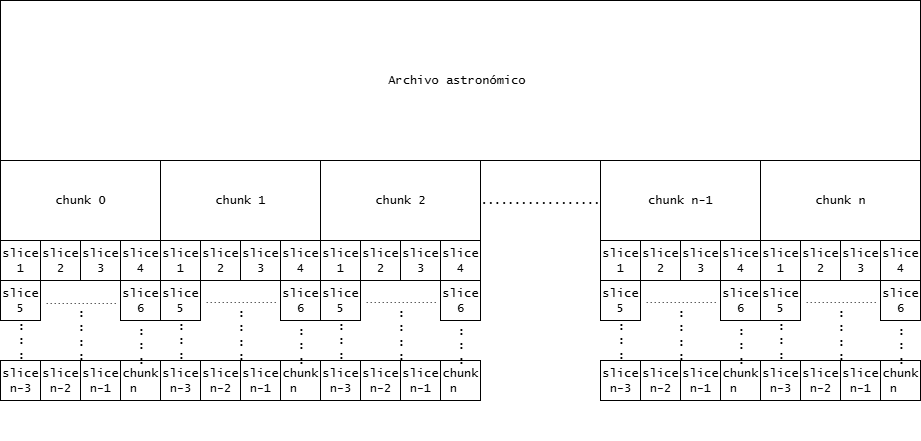
\includegraphics[width=0.9\textwidth]{figures/sistema-chunks.png}
\caption[Esquema de chunks y slices]{Esquema de un archivo astronómico dividido en chunks y slices, ilustrando el concepto de procesamiento con solapamiento. Fuente: Elaboración propia.}
\label{fig:sistema-chunks}
\end{figure}

\subsubsection{Gestión inteligente de memoria y GPU}\label{sec:gpu-memory}

La gestión eficiente de recursos computacionales constituye una mejora fundamental que diferencia DRAFTS++ del prototipo original, el cual carecía de mecanismos sofisticados para la gestión de memoria y recursos GPU. Esta sección define los límites operativos y políticas (presupuestos de RAM/VRAM, limpieza determinística, \textit{fallback} a CPU) que condicionan el plan de \emph{chunk}/\emph{slice} de la Sección \ref{sec:chunk-slice-planning} y el comportamiento en ejecución de la Sección \ref{sec:streaming-continuity}, asegurando estabilidad y rendimiento.

\paragraph{Algoritmo de Planificación de Recursos y Gestión de Memoria Dinámica}

El sistema implementa un \textbf{algoritmo de planificación de recursos} que calcula dinámicamente el tamaño óptimo de \emph{chunks} basándose en la memoria disponible del sistema y las características de los datos. Este algoritmo es fundamental para garantizar que el pipeline pueda procesar observaciones de cualquier tamaño sin desbordamientos de memoria.

El algoritmo de planificación de recursos opera mediante los siguientes pasos:

\begin{enumerate}
    \item \textbf{Cálculo de memoria disponible:} Se determina la memoria RAM disponible del sistema usando \texttt{psutil.virtual\_memory().available}.
    \item \textbf{Estimación de bytes por muestra:} Se calcula el tamaño en bytes que ocupará cada muestra después de la decimación espectral.
    \item \textbf{Aplicación de presupuesto de memoria:} Se reserva un porcentaje de la memoria disponible (típicamente 25\%) para operaciones de \emph{overhead} y estabilidad del sistema.
    \item \textbf{Cálculo de tamaño máximo de chunk:} Se determina el número máximo de muestras que pueden procesarse en un solo \emph{chunk} sin exceder el presupuesto de memoria.
    \item \textbf{Alineación con longitud de slice:} Se ajusta el tamaño del \emph{chunk} para que sea múltiplo exacto de la longitud de \emph{slice}, garantizando contigüidad perfecta.
\end{enumerate}

La formulación matemática del algoritmo se basa en las siguientes ecuaciones:

\[
\text{bytes\_por\_muestra} = 4 \times \left\lfloor \frac{\text{FREQ\_RESO}}{\text{DOWN\_FREQ\_RATE}} \right\rfloor
\]

donde:
\begin{itemize}
    \item $\text{FREQ\_RESO}$: Número total de canales de frecuencia originales
    \item $\text{DOWN\_FREQ\_RATE}$: Factor de decimación espectral aplicado
    \item El factor $4$: Representa el tamaño en bytes de un valor de punto flotante (32-bit)
\end{itemize}

El cálculo de memoria utilizable se realiza mediante:

\[
\text{memoria\_utilizable} = \frac{\text{memoria\_disponible} \times \text{FRACCION\_MAX\_RAM}}{\text{FACTOR\_OVERHEAD}}
\]

donde:
\begin{itemize}
    \item $\text{memoria\_disponible}$: Memoria RAM disponible del sistema en bytes
    \item $\text{FRACCION\_MAX\_RAM}$: Fracción máxima de memoria a utilizar (típicamente 0.25 = 25\%)
    \item $\text{FACTOR\_OVERHEAD}$: Factor de seguridad para operaciones adicionales (típicamente 1.3)
\end{itemize}

El número máximo de muestras por \emph{chunk} se calcula como:

\[
\text{muestras\_max} = \left\lfloor \frac{\text{memoria\_utilizable}}{\text{bytes\_por\_muestra}} \right\rfloor
\]

Finalmente, el tamaño final del \emph{chunk} se alinea con la longitud de \emph{slice}:

\[
\text{chunk\_samples} = \left\lfloor \frac{\text{muestras\_max}}{\text{slice\_len}} \right\rfloor \times \text{slice\_len}
\]

Este algoritmo garantiza que cada \emph{chunk} sea procesable con la memoria disponible mientras mantiene la eficiencia computacional y la contigüidad temporal de los datos.

\begin{algorithm}[H]
\caption{Planificación de Recursos y Gestión de Memoria Dinámica}
\label{alg:resource-planning}
\begin{algorithmic}[1]
\Require Metadatos del archivo (FREQ\_RESO, DOWN\_FREQ\_RATE, FILE\_LENG)
\Ensure Tamaño óptimo de chunk en muestras

\State \textbf{INICIO}
\State Obtener memoria disponible: $\text{mem\_available} = \text{psutil.virtual\_memory().available}$
\State Calcular canales decimados: $\text{channels\_ds} = \lfloor \frac{\text{FREQ\_RESO}}{\text{DOWN\_FREQ\_RATE}} \rfloor$
\State Calcular bytes por muestra: $\text{bytes\_per\_sample} = 4 \times \text{channels\_ds}$

\If{archivo completo cabe en memoria}
    \State $\text{chunk\_samples} = \text{total\_samples\_decimated}$
    \State \textbf{RETORNAR} $\text{chunk\_samples}$
\Else
    \State Calcular memoria utilizable: $\text{usable\_mem} = \frac{\text{mem\_available} \times 0.25}{1.3}$
    \State Calcular muestras máximas: $\text{max\_samples} = \lfloor \frac{\text{usable\_mem}}{\text{bytes\_per\_sample}} \rfloor$
    \State Alinear con slice\_len: $\text{chunk\_samples} = \lfloor \frac{\text{max\_samples}}{\text{slice\_len}} \rfloor \times \text{slice\_len}$
    \If{$\text{chunk\_samples} = 0$}
        \State $\text{chunk\_samples} = \text{slice\_len}$ \Comment{Chunk mínimo}
            \EndIf
\EndIf

\State Validar parámetros calculados
\State \textbf{RETORNAR} $\text{chunk\_samples}$
\State \textbf{FIN}
\end{algorithmic}
\end{algorithm}

\paragraph{Gestión Inteligente de Memoria GPU}

El sistema implementa estrategias avanzadas para la gestión de memoria GPU (VRAM) que optimizan el uso de recursos CUDA y previenen desbordamientos de memoria durante el procesamiento intensivo de dedispersión y detección. A diferencia del prototipo original que carecía de gestión de memoria GPU, DRAFTS++ incluye mecanismos de monitoreo, limpieza automática y fallback a CPU cuando es necesario.

La gestión de memoria GPU opera mediante los siguientes componentes:

\begin{enumerate}
    \item \textbf{Monitoreo de VRAM:} Se implementa telemetría en tiempo real del uso de memoria GPU para detectar situaciones de memoria insuficiente antes de que causen fallos.
    \item \textbf{Limpieza Automática:} Se ejecuta limpieza determinística de tensores y buffers GPU después de cada operación para liberar memoria no utilizada.
    \item \textbf{Fallback a CPU:} Se implementa un mecanismo de fallback automático que transfiere operaciones a CPU cuando la memoria GPU es insuficiente.
    \item \textbf{Contexto de GPU:} Se utiliza un contexto manager que suprime mensajes técnicos de CUDA y maneja errores de manera elegante.
\end{enumerate}

Esta implementación garantiza que el pipeline sea robusto ante diferentes configuraciones de hardware y pueda adaptarse dinámicamente a las limitaciones de memoria disponibles.

\paragraph{Optimización de Recursos Computacionales}

El sistema incluye algoritmos de optimización que ajustan dinámicamente el uso de recursos en función de las características de los datos y la disponibilidad del sistema. Esta optimización incluye:

\begin{enumerate}
    \item \textbf{Balanceado de carga:} Distribución inteligente de operaciones entre CPU y GPU según la disponibilidad de recursos.
    \item \textbf{Gestión de garbage collection:} Liberación proactiva de memoria no utilizada para mantener un uso eficiente de recursos.
    \item \textbf{Telemetría de rendimiento:} Monitoreo continuo del uso de recursos para optimización dinámica.
    \item \textbf{Configuración adaptativa:} Ajuste automático de parámetros de procesamiento basado en las capacidades del sistema.
\end{enumerate}

Esta aproximación integral a la gestión de recursos representa una mejora fundamental que establece las bases para un sistema productivo capaz de operar eficientemente en diferentes entornos computacionales y escalar a observaciones de gran tamaño.


\subsubsection{Integración y Automatización del Workflow de Modelos de DRAFTS}

La etapa de procesamiento integrado representa el núcleo computacional más sofisticado del pipeline DRAFTS++, donde se materializa la convergencia entre ingeniería de software avanzada y la integración automatizada de los modelos de deep learning existentes en DRAFTS-main. Esta sección detalla cómo se procesan los datos astronómicos para identificar y clasificar candidatos FRB utilizando los modelos CenterNet y ResNet18 de manera integrada, automatizada y eficiente dentro de un flujo de trabajo unificado.

A diferencia del prototipo DRAFTS-main que ejecutaba los modelos de detección y clasificación como etapas separadas y desacopladas, DRAFTS++ implementa un sistema integrado que automatiza la orquestación de estos modelos, combinando detección de objetos, clasificación binaria y validación científica en un flujo unificado y optimizado. Esta aproximación elimina las limitaciones del procesamiento manual por lotes separado y establece las bases para un sistema productivo capaz de manejar observaciones de larga duración en tiempo real, tal como se conceptualizó originalmente en el workflow de DRAFTS.

El procesamiento integrado opera mediante tres pilares fundamentales: (i) integración automatizada del modelo CenterNet para detección de candidatos FRB, (ii) orquestación en flujo del modelo ResNet18 para clasificación binaria, y (iii) validación física y temporal que asegura la coherencia científica de las detecciones. Esta arquitectura integrada representa una mejora significativa sobre el prototipo original, que carecía de integración coherente entre estas etapas y requería intervención manual para coordinar los modelos.

\begin{figure}[H]
\centering
\resizebox{\textwidth}{!}{%
\begin{tikzpicture}[
    node distance=0.8cm and 1.4cm,
    stage/.style={rectangle, draw, fill=blue!20, text width=2.0cm, text centered, minimum height=0.7cm, font=\scriptsize},
    model/.style={rectangle, draw, fill=green!20, text width=1.8cm, text centered, minimum height=0.6cm, font=\scriptsize},
    validation/.style={rectangle, draw, fill=orange!20, text width=1.8cm, text centered, minimum height=0.6cm, font=\scriptsize},
    arrow/.style={-Stealth, thick},
    dataflow/.style={-Stealth, thick, dashed, blue}
]

% Entrada
\node[stage] (input) {Imagen\\DM-tiempo};

% CenterNet
\node[model, right=of input] (centernet) {CenterNet\\Detección};

% ResNet18
\node[model, right=of centernet] (resnet) {ResNet18\\Clasificación};

% Validación
\node[validation, right=of resnet] (validation) {Validación\\Física/Temporal};

% Salida
\node[stage, right=of validation] (output) {Candidatos\\Validados};

% Flujo principal
\draw[arrow] (input) -- (centernet);
\draw[arrow] (centernet) -- (resnet);
\draw[arrow] (resnet) -- (validation);
\draw[arrow] (validation) -- (output);

% Etiquetas de datos
\node[above=0.2cm of centernet] {\tiny Candidatos $(DM, t, box)$};
\node[above=0.2cm of resnet] {\tiny Probabilidad $p$};
\node[above=0.2cm of validation] {\tiny Métricas SNR, $t_{abs}$};

\end{tikzpicture}%
}
\caption[Workflow integrado DRAFTS++]{Workflow integrado y automatizado de DRAFTS++: procesamiento secuencial desde detección con CenterNet, clasificación con ResNet18, hasta validación física y temporal, eliminando la necesidad de procesamiento manual por lotes separado del prototipo original.}
\label{fig:integrated-workflow}
\end{figure}
\paragraph{Integración Automatizada del Modelo CenterNet}

El sistema de detección integra el modelo CenterNet existente en DRAFTS-main, una arquitectura de deep learning especializada en detección de objetos, que fue previamente entrenada para identificar candidatos FRB en imágenes DM-tiempo. La contribución de DRAFTS++ no radica en el desarrollo o entrenamiento de este modelo, sino en la implementación de la infraestructura de software necesaria para embeber, ejecutar y orquestar este modelo de manera automatizada dentro del pipeline de streaming.

CenterNet opera mediante la detección de objetos como puntos centrales en el espacio de la imagen, eliminando la necesidad de anclas y procesos de supresión no máxima (NMS). Esta aproximación es particularmente efectiva para detectar transientes rápidos como FRBs, donde la forma y localización precisa son críticas para la validación científica posterior. DRAFTS++ proporciona la infraestructura de software para ejecutar este modelo de manera eficiente y automática.

El algoritmo de integración y ejecución de CenterNet en DRAFTS++ se implementa mediante los siguientes pasos:

\begin{enumerate}
    \item \textbf{Preprocesamiento de imagen:} La imagen DM-tiempo se normaliza y redimensiona a 512×512 píxeles, aplicando normalización estadística y corrección de color para optimizar la entrada del modelo pre-entrenado.
    \item \textbf{Carga y ejecución del modelo:} Se carga el modelo CenterNet pre-entrenado desde los checkpoints existentes en DRAFTS-main y se ejecuta la inferencia sobre la imagen preprocesada.
    \item \textbf{Procesamiento de salidas:} El modelo genera tres mapas de salida: mapa de calor $H$ (centros de objetos), regresión de tamaño $WH$ (dimensiones), y regresión de desplazamiento $OFF$ (correcciones de posición).
    \item \textbf{Post-procesamiento y extracción de candidatos:} Se aplica supresión no máxima adaptada y filtrado por confianza para generar las detecciones finales, extrayendo coordenadas DM-tiempo de los candidatos detectados.
\end{enumerate}

La formulación matemática del modelo CenterNet se basa en las siguientes ecuaciones:

El mapa de calor se genera mediante:

\[
H_{x,y} = \sigma\left(\sum_{i=1}^{N} \exp\left(-\frac{(x - x_i)^2 + (y - y_i)^2}{2\sigma^2}\right)\right)
\]

donde:
\begin{itemize}
    \item $H_{x,y}$: Valor del mapa de calor en la posición $(x,y)$
    \item $N$: Número de objetos en la imagen
    \item $(x_i, y_i)$: Posición central del objeto $i$
    \item $\sigma$: Parámetro de dispersión gaussiana (típicamente 2.0)
    \item $\sigma(\cdot)$: Función de activación sigmoide
\end{itemize}

La regresión de tamaño predice las dimensiones del objeto mediante:

\[
(w, h) = f_{wh}(F_{x_c, y_c})
\]

donde $f_{wh}$ es una función aprendida que mapea las características locales $F_{x_c, y_c}$ a las dimensiones del objeto.

La regresión de desplazamiento calcula la corrección de posición:

\[
(\Delta x, \Delta y) = f_{off}(F_{x_c, y_c})
\]

donde $f_{off}$ predice el desplazamiento respecto al centro del píxel más cercano.

\begin{algorithm}[H]
\caption{Detección de Candidatos FRB con CenterNet}
\label{alg:centernet-detection}
\begin{algorithmic}[1]
\Require Imagen DM-tiempo $I$, modelo CenterNet entrenado
\Ensure Lista de candidatos con coordenadas y confianza

\State \textbf{INICIO}
\State Normalizar imagen: $I_{norm} = \text{normalize}(I)$
\State Redimensionar a 512×512: $I_{resized} = \text{resize}(I_{norm})$
\State Convertir a tensor: $T = \text{to\_tensor}(I_{resized})$

\State \textbf{Inferencia del modelo}
\State $H, WH, OFF = \text{model}(T)$ \Comment{Mapas de calor, tamaño y desplazamiento}
\State Aplicar sigmoide al mapa de calor: $H = \sigma(H)$

\State \textbf{Post-procesamiento}
\State Extraer picos locales: $\text{peaks} = \text{find\_peaks}(H, \text{threshold}=\theta)$
\For{cada pico $p$ en peaks}
    \State $(x_c, y_c) = \text{coordenadas}(p)$
    \State $(w, h) = WH[x_c, y_c]$ \Comment{Regresión de tamaño}
    \State $(\Delta x, \Delta y) = OFF[x_c, y_c]$ \Comment{Regresión de desplazamiento}
    \State Calcular caja delimitadora: $box = [x_c + \Delta x - w/2, y_c + \Delta y - h/2, x_c + \Delta x + w/2, y_c + \Delta y + h/2]$
    \State Calcular DM y tiempo: $(DM, t) = \text{convert\_to\_physical}(box)$
    \State Agregar candidato: $\text{candidates.append}(DM, t, \text{confidence}(p))$
\EndFor

\State \textbf{RETORNAR} candidates
\State \textbf{FIN}
\end{algorithmic}
\end{algorithm}
\paragraph{Orquestación Automatizada del Modelo ResNet18}

El sistema de clasificación integra el modelo ResNet18 existente en DRAFTS-main, una arquitectura de red neuronal residual previamente entrenada para clasificación binaria de FRBs, que opera en tiempo real durante el procesamiento, evaluando cada candidato detectado por CenterNet para determinar si representa un FRB genuino o ruido. La contribución de DRAFTS++ radica en la automatización de la orquestación entre los modelos, eliminando la necesidad de procesamiento manual por lotes separado.

La clasificación binaria se basa en la extracción de características de patches dedispersados correspondientes a cada candidato detectado por CenterNet. El modelo ResNet18 utiliza una arquitectura residual previamente entrenada para procesar imágenes de FRBs, específicamente diseñada para distinguir entre transientes genuinos y artefactos instrumentales. DRAFTS++ proporciona la infraestructura de software para ejecutar este modelo de manera automatizada y en flujo continuo.

El algoritmo de orquestación y ejecución de ResNet18 en DRAFTS++ opera mediante los siguientes pasos:

\begin{enumerate}
    \item \textbf{Extracción de patch:} Se extrae una región de interés (ROI) alrededor de cada candidato detectado por CenterNet en la imagen DM-tiempo.
    \item \textbf{Dedispersión:} Se aplica dedispersión al patch utilizando el DM detectado para obtener la señal temporal integrada.
    \item \textbf{Preprocesamiento:} Se normaliza el patch dedispersado aplicando corrección de tendencia y normalización estadística para optimizar la entrada del modelo pre-entrenado.
    \item \textbf{Carga y ejecución del modelo:} Se carga el modelo ResNet18 pre-entrenado desde los checkpoints existentes en DRAFTS-main y se ejecuta la inferencia sobre el patch preprocesado.
    \item \textbf{Interpretación de probabilidades:} Se interpreta la salida del modelo para obtener la probabilidad intrínseca de pertenencia a la clase FRB, tal como se visualiza en el workflow original de DRAFTS.
    \item \textbf{Decisión automatizada:} Se aplica un umbral de confianza configurable para clasificar automáticamente el candidato como "BURST" o "NO BURST".
\end{enumerate}

La formulación matemática del proceso de clasificación se basa en:

El preprocesamiento del patch se realiza mediante:

\[
P_{norm} = \frac{P - \mu_P}{\sigma_P} \cdot \frac{1}{\text{mean}(P)} + 1
\]

donde:
\begin{itemize}
    \item $P$: Patch original extraído
    \item $\mu_P, \sigma_P$: Media y desviación estándar del patch
    \item $P_{norm}$: Patch normalizado
\end{itemize}

La normalización final se aplica mediante:

\[
P_{final} = \frac{\text{clip}(P_{norm}, v_{min}, v_{max}) - v_{min}}{v_{max} - v_{min}}
\]

donde $v_{min}$ y $v_{max}$ son los percentiles 5\% y 95\% del patch, respectivamente.

La probabilidad de clasificación se calcula mediante:

\[
p = \sigma(W \cdot \phi(P_{final}) + b)
\]

donde:
\begin{itemize}
    \item $p$: Probabilidad de pertenencia a la clase FRB
    \item $\sigma$: Función de activación sigmoide
    \item $W, b$: Pesos y sesgo de la capa de clasificación
    \item $\phi(P_{final})$: Características extraídas por la red convolucional
\end{itemize}

La decisión de clasificación se realiza mediante:

\[
\text{Clase} = \begin{cases} 
\text{BURST} & \text{si } p \geq \theta_{class} \\
\text{NO BURST} & \text{si } p < \theta_{class}
\end{cases}
\]

donde $\theta_{class}$ es el umbral de confianza configurable (típicamente 0.6).

\begin{algorithm}[H]
\caption{Clasificación Binaria en Flujo}
\label{alg:binary-classification}
\begin{algorithmic}[1]
\Require Candidato $(DM, t, box)$, modelo clasificador, datos originales
\Ensure Probabilidad de FRB y clasificación final

\State \textbf{INICIO}
\State Extraer patch de la imagen DM-tiempo: $P = \text{extract\_patch}(box)$
\State Aplicar dedispersión: $P_{dedisp} = \text{dedisperse}(P, DM)$
\State Normalizar patch: $P_{norm} = \frac{P_{dedisp} - \mu}{\sigma} \cdot \frac{1}{\text{mean}(P_{dedisp})} + 1$
\State Aplicar clipping: $v_{min}, v_{max} = \text{percentiles}(P_{norm}, [5, 95])$
\State Normalización final: $P_{final} = \frac{\text{clip}(P_{norm}, v_{min}, v_{max}) - v_{min}}{v_{max} - v_{min}}$

\State \textbf{Clasificación}
\State Convertir a tensor: $T = \text{to\_tensor}(P_{final}[None, None, :, :])$
\State Inferencia: $logits = \text{classifier\_model}(T)$
\State Calcular probabilidad: $p = \text{softmax}(logits)[0, 1]$

\If{$p \geq \theta_{class}$}
    \State $\text{clase} = \text{BURST}$
\Else
    \State $\text{clase} = \text{NO BURST}$
\EndIf

\State \textbf{RETORNAR} $(p, \text{clase})$
\State \textbf{FIN}
\end{algorithmic}
\end{algorithm}
\paragraph{Validación Física y Temporal Integrada}

El sistema de validación implementa verificaciones científicas robustas que aseguran la coherencia física y temporal de los candidatos detectados. Esta validación integrada representa una mejora fundamental sobre el prototipo original, que carecía de verificaciones sistemáticas de calidad.

La validación física se basa en el cálculo de métricas SNR (Signal-to-Noise Ratio) utilizando técnicas de análisis espectral robustas. Se implementa un algoritmo de detección de picos basado en filtrado adaptado que identifica señales significativas en el ruido de fondo.

La validación temporal garantiza la precisión en la localización temporal de los eventos, calculando timestamps absolutos con correcciones por chunk, slice y offset de muestreo. Esta precisión temporal es crucial para la validación científica posterior y la correlación con observaciones independientes.

El algoritmo de validación opera mediante los siguientes pasos:

\begin{enumerate}
    \item \textbf{Cálculo de SNR:} Se calcula el SNR del candidato en la región detectada y en el patch dedispersado.
    \item \textbf{Validación de DM:} Se verifica que el DM detectado esté dentro de rangos físicamente plausibles.
    \item \textbf{Cálculo de tiempo absoluto:} Se calcula el timestamp absoluto con correcciones por chunk y slice.
    \item \textbf{Validación de anchura:} Se estima la anchura temporal del pulso mediante análisis espectral.
    \item \textbf{Validación de coherencia:} Se verifica la consistencia entre las métricas calculadas.
\end{enumerate}

La formulación matemática del cálculo de SNR se basa en:

El SNR se calcula mediante análisis espectral PRESTO-style:

\[
\text{SNR} = \max_w \frac{\text{conv}(s, \text{boxcar}(w))}{\sqrt{w}}
\]

donde:
\begin{itemize}
    \item $s$: Serie temporal dedispersada
    \item $\text{boxcar}(w)$: Kernel de convolución de anchura $w$
    \item $\text{conv}(\cdot, \cdot)$: Operación de convolución
    \item El máximo se toma sobre anchuras $w \in \{1, 2, 3, 4, 6, 9, 14, 20, 30\}$
\end{itemize}

El cálculo de tiempo absoluto se realiza mediante:

\[
t_{abs} = t_{chunk} + t_{slice} + t_{offset} + t_{peak}
\]

donde:
\begin{itemize}
    \item $t_{chunk}$: Tiempo de inicio del chunk
    \item $t_{slice}$: Offset temporal del slice dentro del chunk
    \item $t_{offset}$: Offset de muestreo dentro del slice
    \item $t_{peak}$: Posición del pico dentro del patch dedispersado
\end{itemize}

La validación de DM se realiza mediante:

\[
\text{DM}_{valid} = \begin{cases} 
\text{True} & \text{si } 0 < \text{DM} < \text{DM}_{max} \\
\text{False} & \text{en otro caso}
\end{cases}
\]

donde $\text{DM}_{max}$ es el máximo DM físicamente plausible (típicamente 2000 pc/cm³).

\begin{algorithm}[H]
\caption{Validación Física y Temporal Integrada}
\label{alg:physical-temporal-validation}
\begin{algorithmic}[1]
\Require Candidato $(DM, t, box)$, patch dedispersado, metadatos temporales
\Ensure Métricas de validación y flag de aceptación

\State \textbf{INICIO}
\State Calcular SNR en región candidata: $\text{SNR}_{raw} = \text{compute\_snr}(box)$
\State Calcular SNR en patch dedispersado: $\text{SNR}_{dedisp} = \text{compute\_snr}(patch)$
\State Validar DM: $\text{DM}_{valid} = (0 < DM < 2000)$

\State \textbf{Cálculo de tiempo absoluto}
\State $t_{chunk} = \text{chunk\_start\_sample} \times \text{TIME\_RESO}$
\State $t_{slice} = \text{slice\_start\_idx} \times \text{TIME\_RESO} \times \text{DOWN\_TIME\_RATE}$
\State $t_{offset} = t \times \text{TIME\_RESO} \times \text{DOWN\_TIME\_RATE}$
\State $t_{peak} = \text{peak\_idx} \times \text{TIME\_RESO} \times \text{DOWN\_TIME\_RATE}$
\State $t_{abs} = t_{chunk} + t_{slice} + t_{offset} + t_{peak}$

\State \textbf{Estimación de anchura}
\State $width\_profile = \text{compute\_width\_profile}(patch)$
\State $width\_ms = \text{width\_profile}[\text{peak\_idx}] \times \text{TIME\_RESO} \times \text{DOWN\_TIME\_RATE} \times 1000$

\State \textbf{Validación de coherencia}
\If{$\text{SNR}_{dedisp} \geq \text{SNR}_{threshold}$ y $\text{DM}_{valid}$ y $width\_ms > 0$}
    \State $\text{validated} = \text{True}$
\Else
    \State $\text{validated} = \text{False}$
\EndIf

\State \textbf{RETORNAR} $(\text{SNR}_{raw}, \text{SNR}_{dedisp}, t_{abs}, width\_ms, \text{validated})$
\State \textbf{FIN}
\end{algorithmic}
\end{algorithm}

Esta implementación integrada de detección, clasificación y validación representa una mejora arquitectónica fundamental que establece las bases para un sistema productivo robusto, capaz de procesar observaciones de larga duración con precisión científica y eficiencia computacional optimizada. La contribución clave de DRAFTS++ radica en la automatización y orquestación de los modelos existentes de DRAFTS, transformando un workflow conceptual en un sistema operativo que funciona tal como se visualizó originalmente en el diseño de DRAFTS, con detección y clasificación automatizadas y probabilidades intrínsecas integradas en el flujo de trabajo.


% =============================================================
% Bloque 2: Sólo títulos y subtítulos (estructura)
% =============================================================
\subsection{Bloque 2: Extensión a Alta Frecuencia - Cuatro Líneas de Investigación}

Este bloque explora estrategias metodológicas para extender las capacidades de detección hacia regímenes de alta frecuencia (30-100 GHz), donde las firmas dispersivas tradicionales se atenúan significativamente. La detección de FRBs en el régimen milimétrico presenta desafíos fundamentales que requieren aproximaciones metodológicas diferenciadas.

A estas frecuencias, la dispersión temporal se atenúa significativamente debido a la dependencia cuadrática inversa con la frecuencia, resultando en firmas dispersivas que pueden ser indistinguibles del ruido instrumental en resoluciones temporales típicas. Este bloque presenta cuatro líneas de investigación complementarias que abordan diferentes aspectos del desafío de detección en el espectro milimétrico.

\subsubsection{Línea 1: Validación de DRAFTS++ sin modificaciones}

Esta línea constituye una extensión natural del Bloque 1: se emplea \textbf{exactamente el mismo DRAFTS++ sin modificaciones}, preservando la arquitectura y el \emph{workflow} clásico (DM–tiempo para propuesta y red de clasificación para decisión), con el propósito de \textit{medir su capacidad base} en regímenes de alta frecuencia. El interés es doble: (i) establecer la sensibilidad y robustez mínima alcanzable sin introducir nuevas heurísticas ni rutas alternativas, y (ii) cuantificar objetivamente el punto a partir del cual las estrategias específicas de alta frecuencia (Línea 2) superan al flujo original en eficacia operativa. El criterio físico de resolubilidad se expresa mediante el retardo dispersivo máximo entre los extremos de banda,
\[
\Delta t_{\mathrm{ms}} = 4.148808 \times 10^{3}\,\, \mathrm{DM}\,\big(\nu_{\mathrm{low}}^{-2}-\nu_{\mathrm{high}}^{-2}\big),
\]
comparado con la resolución temporal efectiva $t_{\mathrm{samp}}$. Cuando $\Delta t_{\mathrm{ms}} > \alpha\, t_{\mathrm{samp}}$ (con $\alpha$ de seguridad en el rango 1.5–2.0), el \textit{bow–tie} permanece resoluble y la detección en DM–tiempo sigue siendo pertinente; si $\Delta t_{\mathrm{ms}} \le \alpha\, t_{\mathrm{samp}}$, la firma se comprime y el mapa DM–tiempo pierde contraste, anticipándose una disminución de sensibilidad. La validación consiste, por tanto, en aplicar el flujo sin modificaciones sobre ventanas en las que $\Delta t_{\mathrm{ms}}$ sea resoluble y medir sensibilidad, tasa de falsos positivos y estabilidad temporal del detector; este resultado sirve de referencia objetiva para las estrategias alternativas descritas a continuación.


\subsubsection{Línea 2: Detección por SNR con clasificación binaria en flujo}

Cuando el retardo dispersivo se vuelve comparable o inferior a la resolución temporal, el patrón DM–tiempo pierde contraste y la representación más informativa pasa a ser el perfil temporal. Inspirada en el enfoque clásico de \textbf{PRESTO} \cite{Ransom_PRESTO_Tutorial}, esta línea introduce una \textbf{rama SNR-threshold} dentro del \emph{workflow} original de DRAFTS++: la \textit{propuesta} deja de realizarse con un detector en DM–tiempo y pasa a ejecutarse con un umbral de SNR en la serie temporal; la \textit{decisión} final se mantiene en la red de clasificación binaria ya integrada. Arquitectónicamente, la rama se \textit{activa condicionalmente} cuando el módulo de análisis determina que $\Delta t_{\mathrm{ms}} \le \alpha\, t_{\mathrm{samp}}$ (pérdida de \textit{bow–tie}). Tras proponer con SNR, el flujo \textit{regresa} a la ruta estándar: dedispersión local coherente, clasificación binaria, validaciones físicas y emisión de artefactos estandarizados. Este diseño es atractivo porque (i) conserva el carácter E2E y la unificación de salidas, (ii) reduce el costo de exploración en dominios con poca separabilidad DM–tiempo, y (iii) reutiliza la misma infraestructura de clasificación, auditoría y trazabilidad.

Sea $s(t)$ la serie temporal (obtenida por integración en frecuencia y normalización robusta). La estimación de SNR por filtrado adaptado se define como
\[
\mathrm{SNR}(t) = \max_{w\in\mathcal{W}} \frac{\big(s * b_w\big)(t)}{\sqrt{w}},
\]
donde $b_w$ es un \textit{boxcar} de anchura $w$ y $\mathcal{W}$ un conjunto discreto de anchos. La detección primaria consiste en seleccionar instantes $t_i$ tales que $\mathrm{SNR}(t_i)\ge T$ y $|t_i-t_j|\ge \Delta t_{\min}$ para todo $j\ne i$, lo que evita duplicidades y reagregaciones espurias. Alrededor de cada $t_i$ se construye un parche tiempo–frecuencia centrado en $t_i$ y se evalúa una rejilla local de medidas de dispersión para obtener $\mathrm{DM}^*$ como el valor que maximiza la coherencia temporal dedispersada. Este parche, dedispersado a $\mathrm{DM}^*$ y preprocesado, se somete a la red de clasificación binaria para estimar la probabilidad intrínseca de pertenencia a la clase FRB. Finalmente, se exige consistencia física mínima (por ejemplo, $\mathrm{DM}^*>0$ con incertidumbre acotada y anchura temporal finita) antes de emitir el candidato.

\begin{algorithm}[H]
\caption{Detección híbrida HF: SNR $\rightarrow$ parche dedispersado $\rightarrow$ clasificación}
\label{alg:hf-snr-class}
\begin{algorithmic}[1]
\Require Serie temporal $s(t)$, umbral $T$, separación $\Delta t_{\min}$, conjunto de anchos $\mathcal{W}$, rejilla local de DM
\Ensure Candidatos validados con $\{t_{\mathrm{evt}},\, \mathrm{SNR},\, \mathrm{DM}^*,\, p\}$

\State Normalizar $s(t)$ de forma robusta (tendencia y escala)
\State Calcular $\mathrm{SNR}(t)=\max_{w\in\mathcal{W}} (s*b_w)(t)/\sqrt{w}$
\State Extraer picos $\{t_i\}$ con $\mathrm{SNR}(t_i)\ge T$ y distancia mínima $\Delta t_{\min}$
\For{cada $t_i$}
    \State Construir un parche tiempo–frecuencia centrado en $t_i$
    \State Evaluar la rejilla local de DM y obtener $\mathrm{DM}^*$ por máxima coherencia
    \State Dedispersar y preprocesar el parche a $\mathrm{DM}^*$
    \State Estimar probabilidad binaria $p$ con el clasificador en flujo
    \If{$p$ suficientemente alto y $\mathrm{DM}^*>0$ con anchura temporal finita}
        \State Emitir candidato con $(t_{\mathrm{evt}}\!=\!t_i,\, \mathrm{SNR}(t_i),\, \mathrm{DM}^*,\, p)$
    \EndIf
\EndFor
\end{algorithmic}
\end{algorithm}

\begin{figure}[H]
\centering
\resizebox{\textwidth}{!}{%
\begin{tikzpicture}[
    node distance=0.9cm and 1.6cm,
    stage/.style={rectangle, draw, fill=blue!20, text width=2.3cm, text centered, minimum height=0.7cm, font=\scriptsize},
    decision/.style={diamond, draw, fill=yellow!20, aspect=2, text width=2.4cm, text centered, inner sep=1pt, font=\scriptsize},
    arrow/.style={-Stealth, thick}
]

% Nodos principales
\node[stage] (input) {Archivo\\HF};
\node[decision, right=of input] (cond) {$\Delta t_{\mathrm{ms}} > \alpha\,t_{\mathrm{samp}}$?};
\node[stage, below right=of cond] (snr) {Propuesta por SNR};
\node[stage, above right=of cond] (dmmap) {Propuesta DM--tiempo};
\node[stage, right=3.0cm of snr] (dedisp) {Dedispersión local};
\node[stage, right=of dedisp] (clf) {Clasificación Binaria};
\node[stage, right=of clf] (val) {Validación Física};
\node[stage, right=of val] (out) {Artefactos\\Estandarizados};

% Flujo
\draw[arrow] (input) -- (cond);
\draw[arrow] (cond) -- node[above] {Sí} (dmmap);
\draw[arrow] (cond) -- node[below] {No} (snr);
\draw[arrow] (snr) -- (dedisp);
\draw[arrow] (dmmap) |- (dedisp);
\draw[arrow] (dedisp) -- (clf);
\draw[arrow] (clf) -- (val);
\draw[arrow] (val) -- (out);

\end{tikzpicture}}
\caption[Rama SNR en el workflow HF]{Rama SNR-threshold para alta frecuencia integrada en el workflow de DRAFTS++: la condición física activa la propuesta por SNR cuando el \textit{bow–tie} no es resoluble; el flujo vuelve a la ruta estándar para dedispersión local, clasificación y validación.}
\label{fig:hf-snr-branch}
\end{figure}

\subsubsection{Línea 3: Nuevos Plots Característicos}

\subsubsection{Línea 4: Estrategias Alternativas del Autor de DRAFTS}
